\documentclass[10pt]{article}
\usepackage[ngerman]{babel}
\usepackage[utf8]{inputenc}
\usepackage[T1]{fontenc}
\usepackage{amsmath}
\usepackage{amsfonts}
\usepackage{amssymb}
\usepackage[version=4]{mhchem}
\usepackage{stmaryrd}
\usepackage{graphicx}
\usepackage[export]{adjustbox}
\graphicspath{ {./images/} }

\begin{document}
\section*{Teilaufgabe II: Theoretische Informatik}
Aufgabe 1 (Reguläre Sprachen)

[25 PUNKTE]

a) Geben Sie einen regulären Ausdruck an, der die Sprache aller Wörter über dem Alphabet $\{a, b, c\}$ beschreibt, die das Teilwort $a b$ nicht enthalten.

b) Gegeben sei folgender deterministischer endlicher Automat $M$.

\begin{center}
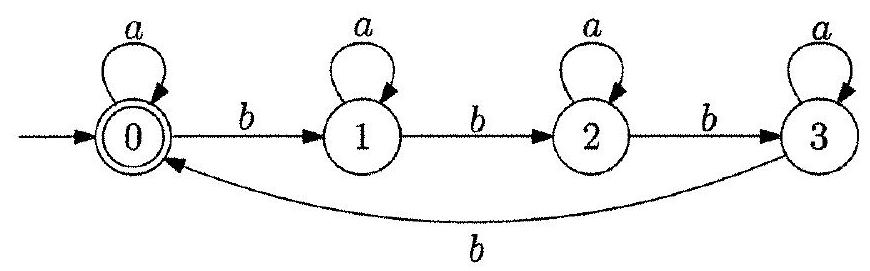
\includegraphics[max width=\textwidth]{2024_05_29_35588a07a9630e5c9887g-2}
\end{center}

Welche Sprache akzeptiert $M$ ? Begründen Sie Ihre Antwort.

c) Konstruieren Sie für folgenden deterministischen endlichen Automaten, der Wörter über dem Alphabet $\{0,1\}$ verarbeitet, den Minimalautomaten, das heißt einen deterministischen endlichen Automaten, der die gleiche Sprache akzeptiert und eine minimale Anzahl an Zuständen benutzt. Erläutern Sie Ihre Vorgehensweise, indem Sie zum Beispiel eine Minimierungstabelle angeben, und geben Sie das Zustandsdiagramm des Minimalautomaten an.

\begin{center}
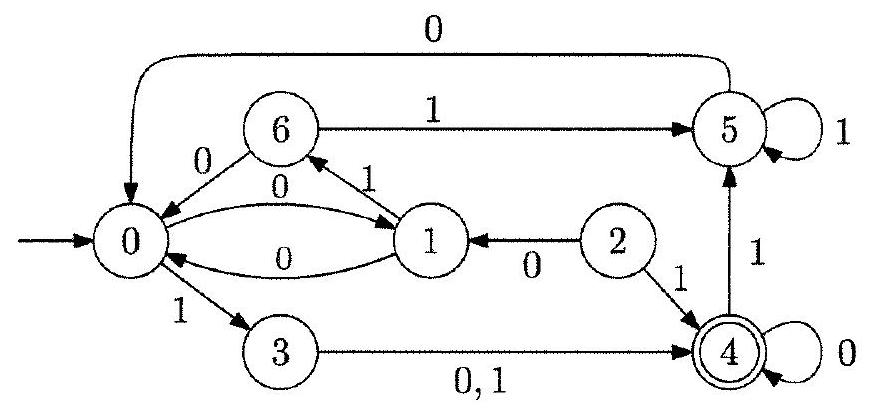
\includegraphics[max width=\textwidth]{2024_05_29_35588a07a9630e5c9887g-2(1)}
\end{center}

Aufgabe 2 (Kontextfreie Sprachen)

a) Sei $G=(V, \Sigma, P, S)$ mit $V=\{S, A, B\}, \Sigma=\{a, b\}$ und folgender Produktionsmenge $P$ :

$$
\begin{aligned}
& S \rightarrow A B \\
& A \rightarrow B B \mid a \\
& B \rightarrow A A|B A| b
\end{aligned}
$$

Prüfen Sie mithilfe des CYK-Algorithmus, ob das Wort $w=a b b a$ in $L(G)$ liegt oder nicht. Falls ja, geben Sie zudem einen Ableitungsbaum für $w$ an. Falls nein, geben Sie alle Teilwörter von $w$ an, die in $L(G)$ liegen.\\
b) i. Sei $K$ eine kontextfreie Sprache und sei $R$ eine reguläre Sprache. Zeigen oder widerlegen Sie, dass $K \cdot R$ im allgemeinen kontextfrei ist.

ii. Sei $K$ kontextfrei und sei $L$ eine Sprache, sodass $K \cdot L$ kontextfrei ist. Zeigen oder widerlegen Sie, dass $L \mathrm{im}$ Allgemeinen kontextfrei ist.

Hinweis: Sie können ohne Beweis verwenden, dass die Sprache $L^{\prime}=\left\{a^{n} b^{m} c^{m} \mid n \leq m\right\}$ nicht kontextfrei ist.

\section*{Aufgabe 3 (Chomsky-Hierarchie)}
[24 PUNKTE]

Sei $\Sigma=\{(),,[]$,$\} ein Alphabet und sei L$ die Sprache der korrekten Klammerausdrücke über $\Sigma$, die von der Grammatik $G=(V, \Sigma, P, S)$ mit $V=\{S\}$ und folgender Produktionsmenge $P$ erzeugt wird:

$$
S \rightarrow(S)|[S]| S S|0|[]
$$

Bestimmen Sie für die folgenden Teilsprachen von $L$ jeweils, ob sie regulär sind und ob sie kontextfrei sind. Beweisen Sie Ihre Antworten. Für jede zutreffende Eigenschaft genügt es, eine geeignete Beschreibung (Grammatik/regulärer Ausdruck) oder die Arbeitsweise eines geeigneten Akzeptors (Automat/Maschine) ohne Korrektheitsbeweis zu anzugeben.

(a) $L_{1}=\{w \in L$ : vor jedem (in $w$ stehen mehr [ als ] $\}$

(b) $L_{2}=\{w \in L$ : auf jede öffnende Klammer folgt direkt eine schließende Klammer $\}$

\section*{Aufgabe 4 (Entscheidbarkeit)}
[26 PUNKTE]

Gegeben sei das Alphabet $\Sigma=\{0,1\}$ und eine Turingmaschine $N$ mit $L(N)=\Sigma^{*}$. Bestimmen Sie für die folgenden Sprachen, ob sie entscheidbar sind und beweisen Sie jeweils Ihre Antwort. Dabei bezeichnet $\langle M\rangle$ die Gödelnummer der Turingmaschine $M$.

(a) $L_{1}=\left\{\langle M\rangle \mid M\right.$ hält auf Eingabe $\langle N\rangle$, benötigt dafür aber mindestens $2^{|\langle N\rangle|}$ Schritte $\}$

(b) $L_{2}=\{\langle M\rangle \mid M$ hält auf Eingabe $\langle N\rangle\}$

(c) $L_{3}=\{\langle M\rangle \mid M$ hält auf mindestens einem Wort, auf welchem $N$ nicht hält $\}$

Aufgabe 5 (Komplexitätstheorie)

[24 PUNKTE]

Sei $G=(V, E)$ ein Graph. Eine Beinahe-3-Färbung von $G$ weist jedem Knoten von $G$ eine der drei Farben $1,2,3 \mathrm{zu}$, sodass für höchstens eine Kante von $G$ beide Endpunkte dieselbe Farbe haben.

(a) Geben Sie einen Graphen an, der eine Beinahe-3-Färbung besitzt, aber keine 3-Färbung. Begründen Sie Ihre Antwort.

(b) Zeigen Sie, dass es NP-vollständig ist, zu entscheiden, ob ein gegebener Graph eine Beinahe3-Färbung besitzt. Dabei dürfen Sie verwenden, dass 3-Färbung NP-vollständig ist.

\section*{Teilaufgabe II: Theoretische Informatik}
\section*{Aufgabe 1 (Konstruktion)}
Sei $M$ ein beliebiger nichtdeterministischer endlicher Automat (NFA), sei $v \in \Sigma^{*}$ und sei $L$ die Sprache $L=\left\{w \in \Sigma^{*} \mid w \in L(M)\right.$ und $w$ enthält $\left.v\right\}$ (Ein Wort $w \in \Sigma^{*}$ enthält $v$, wenn es Wörter $u, u^{\prime} \in \Sigma^{*}$ gibt mit $w=u v u^{\prime}$.).

a) Beschreiben Sie ein allgemeines Verfahren, um $M$ in einen NFA $M^{\prime}$ mit $L\left(M^{\prime}\right)=L \mathrm{zu}$ konvertieren.

b) Führen Sie Ihr Verfahren aus Teilaufgabe a) auf dem folgenden NFA und dem Wort $v=a b$ durch.

\begin{center}
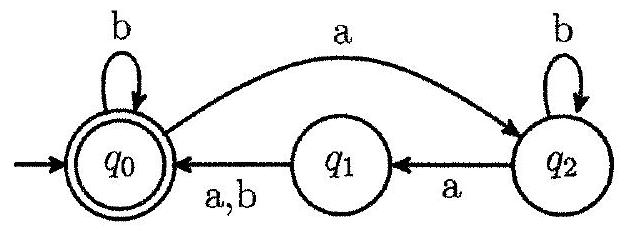
\includegraphics[max width=\textwidth]{2024_05_29_35588a07a9630e5c9887g-4}
\end{center}

\section*{Aufgabe 2 (Minimale DFAs)}
Wir benutzen das Alphabet $\Sigma=\{a, b\}$. Welche der folgenden DFAs sind minimal? Wenn der DFA minimal ist, zeigen Sie es mit Hilfe eines allgemeinen Verfahrens. Wenn der DFA nicht minimal ist, geben Sie einen anderen DFA mit weniger Zuständen an und erklären Sie, warum er äquivalent zum ursprünglichen DFA ist.\\
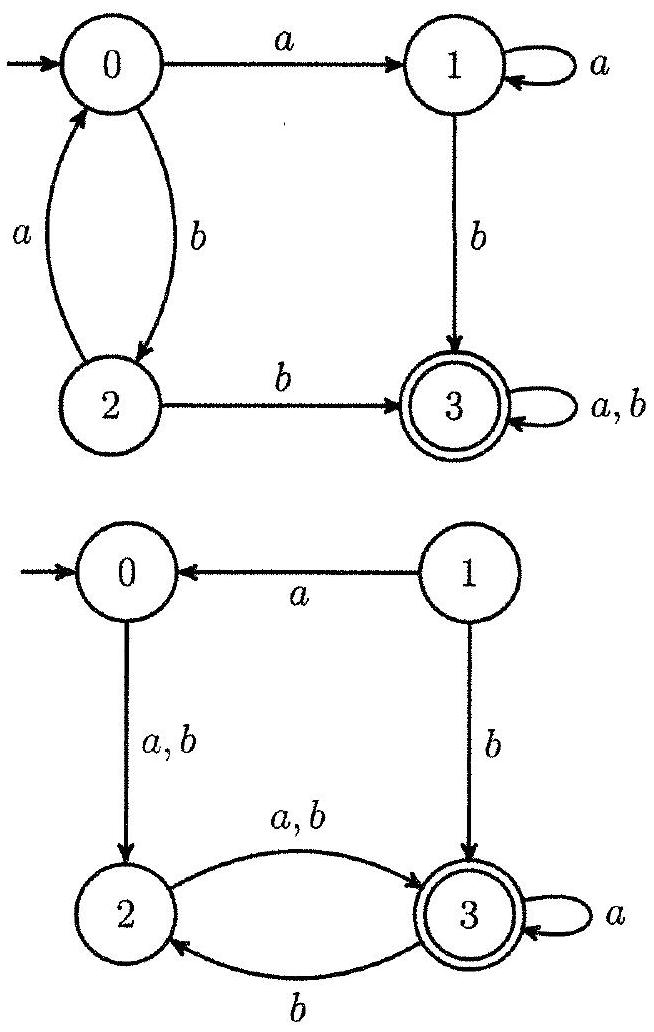
\includegraphics[max width=\textwidth, center]{2024_05_29_35588a07a9630e5c9887g-4(1)}

\begin{center}
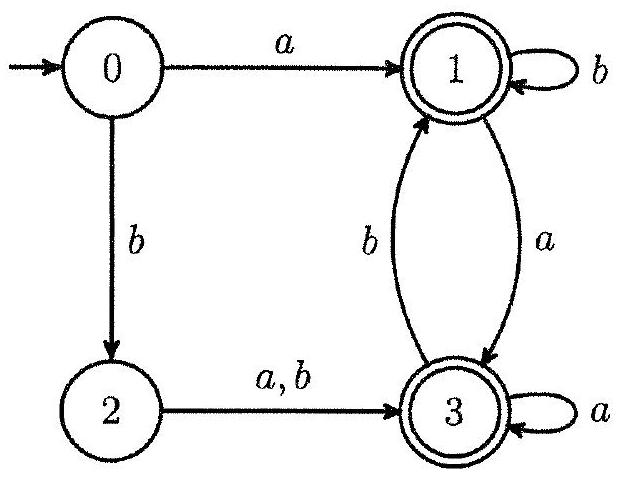
\includegraphics[max width=\textwidth]{2024_05_29_35588a07a9630e5c9887g-5}
\end{center}

Aufgabe 3 (Kontextfreie Grammatiken)

[24 PUNKTE]

Eine kontextfreie Grammatik ist in Chomsky-Normalform (CNF), wenn sämtliche Produktionen die Gestalt $X \rightarrow Y Z$ oder $X \rightarrow a$ besitzen, wobei $X, Y, Z$ Variablen (auch Nichtterminale genannt) und $a$ ein Terminalzeichen ist.

a) Gegeben sei die Grammatik $G=(V, \Sigma, P, S)$ mit $V=\{S, X, Y\}$ und $\Sigma=\{a, b\}$ und folgender Produktionsmenge $P$ :

$$
\begin{aligned}
& S \rightarrow a X Y \\
& X \rightarrow Y \mid \epsilon \\
& Y \rightarrow a S \mid b
\end{aligned}
$$

Geben Sie eine kontextfreie Grammatik $H$ in CNF an mit $L(H)=L(G) \backslash\{\epsilon\}$. Die Grammatik soll höchstens 5 Variablen haben. Erklären Sie Ihren Lösungsweg.

b) Geben Sie eine kontextfreie Grammatik in CNF für die Sprache $\left\{a^{12}\right\}$ an, die höchstens 5 Produktionen verwendet.

Hinweis: Betrachten Sie Produktionen der Form $X \rightarrow Y Y$.

c) Sei $G=(\Sigma, V, S, P)$ eine beliebige Grammatik in CNF. Konstruieren Sie eine kontextfreie Grammatik $H=\left(\Sigma, V^{\prime}, S^{\prime}, P^{\prime}\right)$ mit $L(H)=\{w \in L(G): w$ ist gerade $\}$, d.h. $L(H)$ enthält genau die Wörter aus $L(G)$, deren Länge geradzahlig ist.

Nehmen Sie $V^{\prime}:=\left\{X_{g}, X_{u} \mid X \in V\right\}$ und $S^{\prime}:=S_{g}$. Sie müssen also nur die Menge $P^{\prime}$ der Produktionen von $H$ präzise beschreiben. Erklären Sie die Idee hinter Ihrer Konstruktion.

\section*{Aufgabe 4 (Berechenbarkeit)}
[20 PUNKTE]

Geben Sie an, ob die folgenden Aussagen wahr oder falsch sind. Wenn die jeweilige Aussage wahr ist, beweisen Sie die Aussage; wenn sie falsch ist, geben Sie ein Gegenbeispiel an.

a) Seien $M_{1}, M_{2}$ beliebige Turingmaschinen und sei $L$ eine Sprache mit $L\left(M_{1}\right) \subseteq L \subseteq L\left(M_{2}\right)$. Dann ist $L$ semi-entscheidbar.

b) Seien $L_{1}, L_{2}$ semi-entscheidbar. Dann ist $L_{1} \backslash L_{2}$ semi-entscheidbar.

c) Sei $L$ entscheidbar. Dann ist $L^{\prime}:=\{u v \mid u, v \in L\}$ entscheidbar.

d) Sei $L$ unentscheidbar. Dann ist $L^{\prime}:=\{u \mid \exists v: u v \in L\}$ unentscheidbar.

\section*{Aufgabe 5 (Reduktion)}
[30 PUNKTE]

Eine aussagenlogische Formel ist in konjunktiver Normalform (KNF), wenn sie eine Konjunktion von Disjunktionen von Literalen ist. Z. B. ist $(x \vee y \vee \neg z) \wedge(\neg x \vee \neg y)$ eine KNF-Formel.

Eine Formel ist erfüllbar, wenn sie mindestens eine erfüllende Belegung hat. Zwei Formeln über denselben Variablen sind äquivalent, wenn sie dieselben erfüllenden Belegungen haben, d. h. jede Belegung erfüllt beide Formeln oder keine. Wir betrachten folgende Probleme:

Negierte-KNF-SAT\\
Eingabe: Eine KNF-Formel $F$.\\
Ausgabe: Ist $\neg F$ erfüllbar?

KNF-Nicht-Äquivalenz

Eingabe: Zwei KNF-Formeln $F$ und $G$.

Ausgabe: Sind $F$ und $G$ nicht-äquivalent?

Nehmen Sie $\mathrm{P} \neq \mathrm{NP}$ an. Welche dieser zwei Probleme sind unter dieser Annahme in $\mathrm{P}$ und welche sind NP-vollständig? Begründen Sie Ihre Antwort.


\end{document}